\section{Introdução e Justificativas}\label{Intro}


%=============================================================================
% 							INTRODUÇÃO
%=============================================================================


%INTRODUÇÃO MAIS LONGA: EUA E CRISE
Nos anos 2008 e 2009,
os EUA experimentaram sua maior crise econômica (até então) desde o \textit{crash} de 1929. Essa crise, conhecida como Grande Recessão, teve importantes consequências sociais, econômicas e políticas, mas também impactou o mundo das ideias, com implicações que ainda estão em curso para a teoria econômica. 
%Iniciada como uma crise focalizada no mercado imobiliário americano, a Grande Recessão teve consequências sócio-econômicas devastadoras e implicações para a teoria econômica que ainda estão em curso.  
Por um lado, abalou a macroeconomia \textit{mainstream} ao ponto de a política econômica estar sendo repensada \cite{blanchard_rethinking_2010}, por outro, redirecionou pautas na heterodoxia. 
Distribuição e desigualdade tiveram um novo fôlego \cites{carvalho_personal_2016}{ederer_will_2019} 
enquanto outros trabalhos passaram a enfatizar a importância macroeconômica do consumo das famílias \cites{barba_rising_2009}{brochier_macroeconomics_2017}\footnote{Cabe pontuar que o \textit{mainstream}  também passou a se dedicar ao assunto com destaque ao trabalho de \textcite{piketty_o_2014}.}.
Em paralelo, verificou-se um maior interesse nas implicações macroeconômicas do investimento residencial \cites{teixeira_crescimento_2015}{fiebiger_semi-autonomous_2018} e na relevância de seu financiamento para a macroeconomia contemporânea \cite{jorda_great_2016} e é justamente nessa agenda de pesquisa que essa investigação se insere.

Diante deste contexto, a literatura heterodoxa recente tem se dedicado às consequências macroeconômicas  da ampliação do setor financeiro, do endividamento das firmas  e, mais recentemente, das famílias  \cites{carvalho_income_2014}{hein_demise_2015}{detzer_financialization_2019}.
No entanto, pouca atenção é dada para a composição desses elementos no balanço patrimonial dos bancos.
Tal análise tornou-se possível graças a \textcite{jorda_rate_2019} pelo desenvolvimento de uma base de dados para os anos de 1870--2016 desagregada ao nível do setor bancário de 17 países da OCDE\footnote{São eles: Alemanha, Áustria, Bélgica, Canadá, Dinamarca, Espanha, Estados Unidos, Finlândia, França, Holanda, Itália, Japão, Noruega, Portugal, Reino Unido, Suécia e Suíça. Cabe aqui a menção de que esta base de dados é inédita, está em constante atualização, tem sido pouco explorada e está disponível em \url{http://www.macrohistory.net/data/}.\label{nota_paises}}.
Partindo desses dados, \textcite{jorda_great_2016} identificam que o crescimento recente dos balanços patrimoniais dos bancos é liderado pela concessão de crédito às famílias.
Estes autores também reportam uma priorização do crédito hipotecário  pelos bancos
%as aplicações em imóveis 
cujas implicações precisam ser compreendidas em maior detalhe. 
Em especial, os autores destacam uma tendência de recomposição do balanço patrimonial dos bancos comerciais em que a participação relativa das hipotecas dobra, passando de cerca de 30\% em 1950 para aproximadamente 60\% no período recente. % (ver figura \ref{GraficoJorda}).
Esse aumento sem precedentes da participação das hipotecas e dos imóveis no ativo do balanço patrimonial dos bancos é denominado de ``hipotecarização'' (\textit{mortgaging} no original).

Da revisão bibliográfica, nota-se que a literatura macroeconômica tem investigado os seguintes temas separadamente:  
    mudanças na composição patrimonial dos bancos comerciais; 
    papel do investimento residencial e de bolhas de ativos na dinâmica macroeconômica;
    endividamento, crise  e fragilidade financeira das famílias.
%mercado imobiliário e de crédito; bolhas de ativos e preço dos imóveis; investimento residencial e endividamento das famílias.
A conexão deste recorte específico de temas será aqui denominada de ``macroeconomia imobiliária''.
Esta tese, portanto, tem como objetivo conectar o lado real e financeiro da economia relacionando os impactos, as mudanças e as consequências macroeconômicas do mercado imobiliário tendo em vista elementos teóricos, empíricos e institucionais sob o contexto da hipotecarização. % TODO Marcar: Que tal agora? Suprimi uma frase.
%Dito isso, esta pesquisa busca responder a seguinte pergunta: quais os condicionantes, determinantes e implicações da hipotecarização sobre a dinâmica macroeconômica?
As subseções seguintes exploram diferentes dimensões da aqui denominada macroeconomia imobiliária --- assim como pontuam algumas das lacunas onde esta pesquisa pretende avançar --- são elas: (i) institucionais; (ii) empíricas e; (iii) integração do lado real e financeiro.
%A justificativa desta investigação se deve a uma regularidade do capitalismo contemporâneo já mencionada, mas ainda pouco estudada:  hipotecarização.
%Dada a relevância dos imóveis para a dinâmica macroeconômica, parte-se de uma abordagem multidimensional para contemplar seus principais elementos, são eles: (i) institucionais; (ii) dinâmicos e; (iii) integração do lado real e financeiro.
Cada uma destas frentes será discutida a seguir enquanto os objetivos são apresentados na seção \ref{OBJ}, os procedimentos metodológicos na seção \ref{passos},  o plano de trabalho  se encontra na seção \ref{cronograma} e encerra-se com a proposta de estágio no exterior na seção \ref{BEPE}.

\begin{comment}
Em outras palavras, a presente pesquisa se justifica pela necessidade de uma maior e melhor compreensão do papel macroeconômico dos imóveis e, em especial, da hipotecarização.

\begin{quote}
	\textit{To a large extent the core business model of banks in advanced economies today resembles that of real estate funds: banks are borrowing (short) from the public and capital markets to invest (long) into assets linked to real estate.} [...] \textit{looking more deeply at the composition of bank credit, it becomes clear that the rapid growth of \textbf{mortgage lending} to households has been the \textbf{driving force} behind this remarkable change in the composition of banks' balance sheets} \cite[p.~2, grifos adicionados]{jorda_great_2016}
\end{quote}


Como mencionado, a fronteira tem avançado algumas frentes em paralelo. Uma delas diz respeito a importância das instituições para as relações entre mercado imobiliário, de crédito e endividamento das famílias.
Outra frente trata da importância do investimento residencial para a dinâmica macroeconômica por meio de modelos econométricos.  
Por fim, uma parcela menor direciona esforços para conectar o investimento imobiliário, relação entre famílias e bancos nas teorias de crescimento liderados pela demanda. Esta pesquisa irá avançar nestas direções e suprir algumas das lacunas que serão destacadas adiante.

\begin{figure}[H]
	\centering
	\caption{Participação do empréstimo imobiliário no total do balanço patrimonial dos bancos (1870-2016)}
	\label{GraficoJorda}
	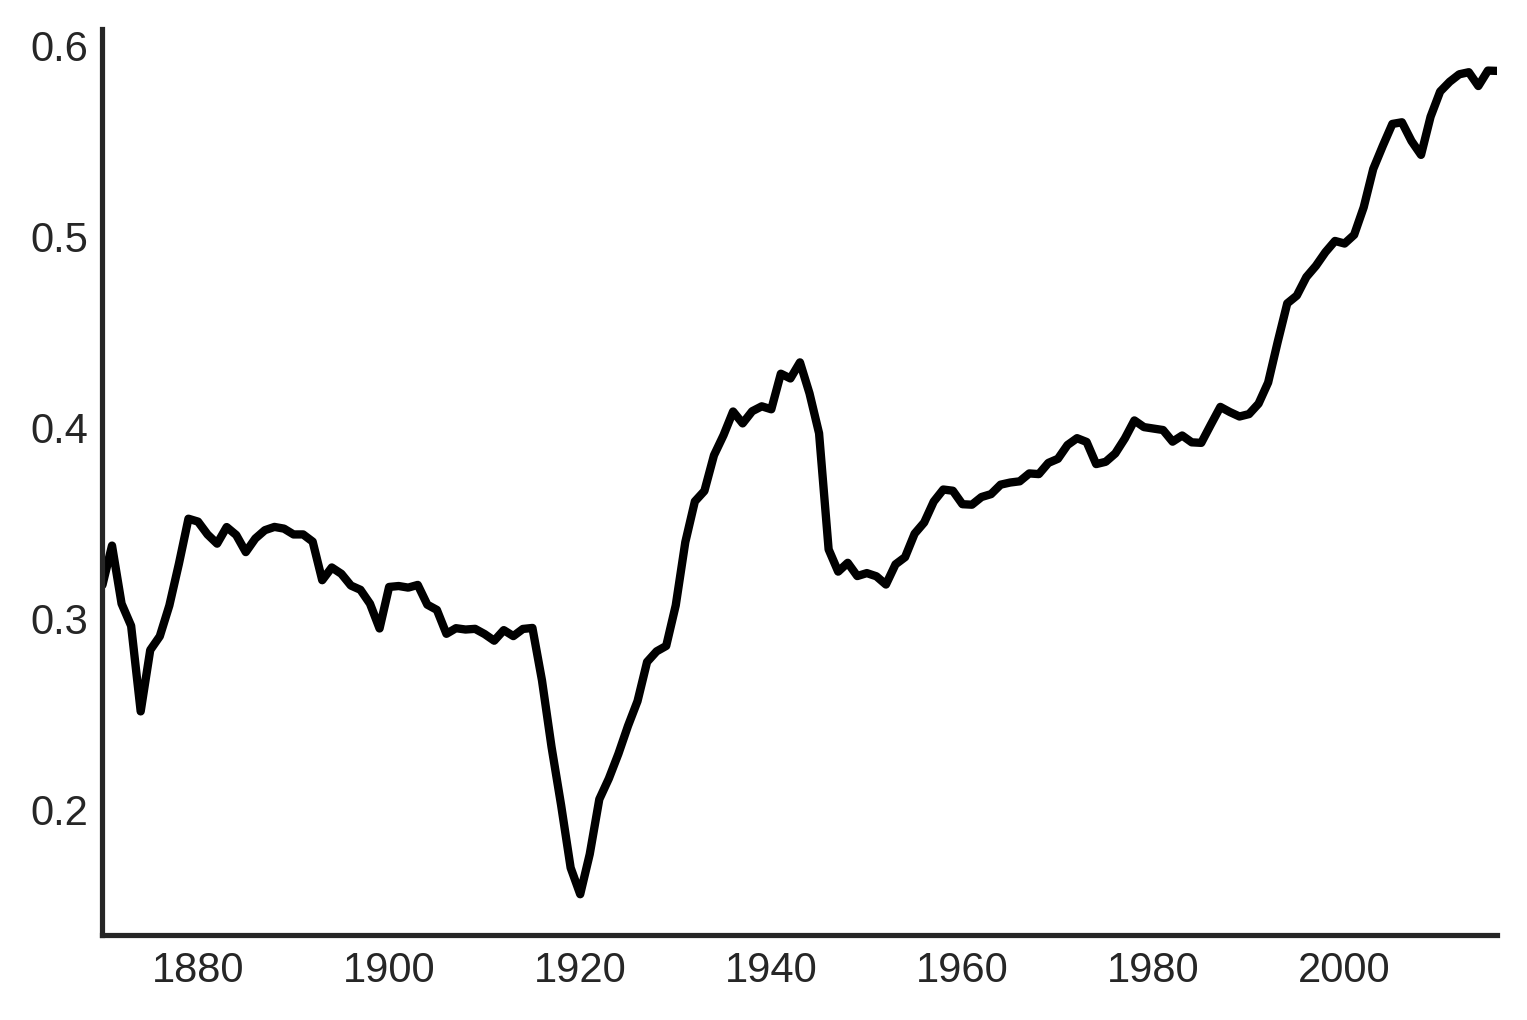
\includegraphics[width=.63\textwidth]{./figs/Jorda_Mean.png}
	\caption*{\textbf{Fonte:} \textcite[p.~10]{jorda_great_2016}}
\end{figure}

\end{comment}




